% !TEX program = xelatex
% !TeX encoding = utf8
% !TeX spellcheck = pl-PL

%%%%%%%%%%%%%%%%%%%%%%%%%%%%%%%%%%%%%%%%%%%%%%%%%%%%%%%%%%%%%%%%%%%%%%%%%%%
% Wybierz rodzaj pracy dyplomowej oraz wydział
% Pick thesis type and faculty
%%%%%%%%%%%%%%%%%%%%%%%%%%%%%%%%%%%%%%%%%%%%%%%%%%%%%%%%%%%%%%%%%%%%%%%%%%%
\documentclass[thesis=inz,faculty=ee]{EE-dyplom} 

% thesis=[inz|mgr|bsc|msc]
%  * inz - praca inżynierska
%  * mgr - praca magisterska
%  * bsc - bachelor thesis
%  * msc - master thesis

% Skróty nazw wydziałów zgodne z domenami internetowymi
% Abbreviations of Faculties according to Internet subdomains
% faculty=[
%	arch,
%	gik,
%	ee,
%	wip
%	]

%%%%%%%%%%%%%%%%%%%%%%%%%%%%%%%%%%%%%%%%%%%%%%%%%%%%%%%%%%%%%%%%%%%%%%%%%%%
% Konfiguracja - do personalizacji
% Configuration - to be personalized
%%%%%%%%%%%%%%%%%%%%%%%%%%%%%%%%%%%%%%%%%%%%%%%%%%%%%%%%%%%%%%%%%%%%%%%%%%%
\instytut{Instytut Sterowania i Elektroniki Przemysłowej}
\kierunek{Informatyka Stosowana}
\specjalnosc{Informatyka Stosowana}
\title{Analiza porównawcza neuronowych wizyjnych algorytmów percepcji głębi}
\engtitle{Comparative analysis of neural vision algorithms for depth perception}
\album{315564}
\author{Patryk Piotrowski}
\promotor{dr inż. Witold Czajewski}
\date{2024}
% \date{\the\year{}}
\miejscowosc{Warszawa}
%\longdate{2077-07-27}

%\grantlicense{TRUE} % [TRUE|FALSE]

%%%%%%%%%%%%%%%%%%%%%%%%%%%%%%%%%%%%%%%%%%%%%%%%%%%%%%%%%%%%%%%%%%%%%%%%%%%
% Streszczenie pracy i abstract.
% In case of thesis in English swap the order - English version goes first.
%%%%%%%%%%%%%%%%%%%%%%%%%%%%%%%%%%%%%%%%%%%%%%%%%%%%%%%%%%%%%%%%%%%%%%%%%%%
\streszczeniepracy{
Streszczenie pracy powinno w zwięzły sposób opisywać to czego dotyczy praca, co jest jej celem, jakie przyjęto założenia, co w ramach pracy zrobiono, co przebadano, jakie rozwiązania zaproponowano i jakie wyniki osiągnięto. Jeśli coś sprawiło jakiś problem, można to także ująć w streszczeniu i skomentować czy udało się ów problem rozwiązać i jak, czy też nie (nic w tym złego, jeśli czegoś się nie udało do końca zrobić). 
\\
Streszczenie nie powinno być przeładowane, powinno mieć około 200 słów i zawierać najważniejsze informacje na temat pracy i najważniejsze osiągnięcia, nie należy więc podawać szczegółowych wyników czy też opisywać struktury pracy - na to miejsce znajduje się w samej pracy.
\\
Streszczenie zwykle pisze się na samym końcu pracy - z oczywistych względów.
\newline
\newline
Przykładowe streszczenie:
\newline
\newline
\noindent\textit{W niniejszej pracy inżynierskiej zaprezentowane zostały próby rozwiązania problemu klasyfikacji poziomu zabrudzenia chodników z wykorzystaniem głębokich sieci neuronowych. Wykorzystując dostępny zbiór zdjęć sklasyfikowanych do sześciu klas poziomu zanieczyszczeń, wygenerowano zrównoważone zbiory: sześcioklasowy oraz trzyklasowy. Następnie wybrano trzy sieci różnego rodzaju, aby sprawdzić ich efektywność w rozróżnianiu poszczególnych, często bardzo zbliżonych do siebie zdjęć. Sieć TResNet została wybrana spośród wiodących sieci w rankingach klasyfikacyjnych. Sieć ShuffleNet V2 została wybrana spośród dostępnych implementacji sieci w ramach popularnej biblioteki OpenMMLab. Sieć PMG została wybrana spośród sieci przygotowanych do rozwiązywania specyficznych problemów klasyfikacyjnych dla obrazów o niewielkich różnicach. Wymienione sieci wytrenowano na wygenerowanych zbiorach i osiągnięto dokładność rzędu 80\% i 90\%, odpowiednio dla problemu sześcio- i trzyklasowego. Najlepszą siecią, w każdym przypadku, okazała się sieć PMG, a wyniki pozostałych sieci były zbliżone.}
} % koniec streszczenia
%%%%%%%%%%%%%%%%%%%%%%%%%%%%%%%%%%%%%%%%%%%%%%%%%%%
\slowakluczowe{istotne, słowa, kluczowe} 
%%%%%%%%%%%%%%%%%%%%%%%%%%%%%%%%%%%%%%%%%%%%%%%%%%%
\thesisabstract{
Należy zadbać oto, by jakość tłumaczenia streszczenia była wyższa niż ta oferowana przez automaty takie jak powszechnie używany \href{https://translate.google.pl/}{https://translate.google.pl/} czy mniej znany, ale czasem lepszy: \href{https://www.deepl.com/translator}{https://www.deepl.com/translator} czy może też \href{https://www.translate.com/}{https://www.translate.com/}. Wszystkie te strony są pomocne i często zgrabnie tłumaczą, ale potrafią też zrobić oczywiste błędy, zwłaszcza w przypadku zdań wielokrotnie złożonych. Warto też skorzystać z serwisu \href{https://www.grammarly.com/}{https://www.grammarly.com}.
\newline
\newline
W miarę poprawny przykład:
\newline
\newline
\textit{This engineering thesis presents an attempt to solve the problem of sidewalk dirt level classification using deep neural networks. Using an available set of images classified into six classes of dirt levels, balanced sets of six classes and three classes were generated. Three networks of different types were then selected to test their effectiveness in discriminating between individual, often very similar, images. TResNet was selected among the leading networks in the classification rankings. The ShuffleNet V2 network was selected from available network implementations within the popular OpenMMLab library. The PMG network was selected from networks prepared to solve specific classification problems for images with small differences. The aforementioned networks were trained on the generated sets and an accuracy of 80\% and 90\% was achieved for the six-class and three-class problem, respectively. The PMG network proved to be the best network, in each case, and the results of the other networks were similar.}
} % end of abstract
%%%%%%%%%%%%%%%%%%%%%%%%%%%%%%%%%%%%%%%%%%%%%%%%%%%
\thesiskeywords{keywords, that, are, indicative}  
%%%%%%%%%%%%%%%%%%%%%%%%%%%%%%%%%%%%%%%%%%%%%%%%%%%

%%%%%%%%%%%%%%%%%%%%%%%%%%%%%%%%%%%%%%%%%%%%%%%%%%%%%%%%%%%%%%%%%%%%%%%%%%%
% Tu zaczyna się dokument
% Here is the beginning of the document
%%%%%%%%%%%%%%%%%%%%%%%%%%%%%%%%%%%%%%%%%%%%%%%%%%%%%%%%%%%%%%%%%%%%%%%%%%%
\begin{document}
    % Strony nagłówkowe
    % Headers
    \frontpages

    % kolejne rozdziały pracy
    % consecutive chapters of the thesis
    \chapter{Wstęp}\label{chap:wstęp}

Sieci neuronowe jako narzędzie przetwarzania informacji są szeroko eksploatowane w celu rozwiązywania problemów niezliczonych sektorów już od wielu dekad\footnote{Początki sieci neuronowych sięgają lat czterdziestych XX wieku \cite{mccullochpitts1943}.}. Ich obecność w tworzonym dziś oprogramowaniu stanowi pomoc dla pracowników branży m.in. medycznej, motoryzacyjnej, ekonomicznej, coraz częściej również rozrywkowej. Rozwój technologii powiązanych z zagadnieniem sztucznej inteligencji następuje niezmiennie w wysokim tempie. Wraz z rozwojem rzeczonej technologii zaczęto implementować neuronowe algorytmy wizji komputerowej umożliwiające przetwarzanie obrazów zarejestrowanych w postaci cyfrowej \cite{tadeusiewiczflasinski1991}. Do tej grupy należą neuronowe wizyjne algorytmy percepcji głębi. Znajdują one zastosowanie między innymi jako fundament autonomicznej mobilności, w systemach rozszerzonej rzeczywistości czy w robotyce. Lepsze zrozumienie głębi sceny widzianej jednym obiektywem pełni w tych obszarach kluczową rolę. Umożliwia reagowanie na przeszkody w czasie rzeczywistym, analizę pod kątem dostępności powierzchni jak również wykonywanie przybliżonych pomiarów. W połączeniu z innymi technikami, takimi jak segmentacja obrazu \cite{minaee2021} polegająca na podziale na charakterystyczne części związane z obiektami widocznymi na obrazie pozwala budować zaawansowane systemy wizyjne.

Algorytmy percepcji głębi stanowią znaczne uproszczenie w dziedzinie pozyskiwania informacji o głębi dwuwymiarowego obrazu, głównie przez wzgląd na charakterystykę pozostałych znanych dotychczas metod, które zakładają posiadanie kosztownej elektroniki\footnote{Na przykład kamery 3D skorelowanej z systemem LIDAR. \cite{dubik1989}} oraz konieczność jej użycia w trakcie wykonywania fotografii podczas gdy zastosowanie algorytmów może mieć miejsce w dowolnym odstępie czasu następującym po utrwaleniu obrazu. Otworzyło to zatem możliwość rozpoznania głębi obrazów nie tylko wykonanych przy pomocy pojedynczego obiektywu, ale również zarejestrowanych historycznie.

Zadanie wizyjnych algorytmów percepcji głębi opartych o sieci neuronowe polega na estymacji odległości każdego pojedynczego zarejestrowanego piksela względem urządzenia rejestrującego na podstawie pojedynczej fotografii wykonanej jednym obiektywem. W zależności od algorytmu wynikowe odległości mogą mieć charakter względny lub metryczny. Realizacja tego zadania polega na przetworzeniu obrazu wejściowego przez warstwy sieci neuronowej odpowiedniej dla architektury danego algorytmu. Ostatecznym wynikiem realizacji tego zadania jest macierz zawierająca wartości odległości dla pojedynczych pikseli. Wizualną reprezentację takiej macierzy stanowi mapa głębi (rys. \ref{fig:depthmap}).

\begin{figure}[H]
        \centering
        \includegraphics[width=0.9\textwidth]{1.jpg}
        \caption{Fotografia i odpowiadająca jej mapa głębi. Źródło: własne}
        \label{fig:depthmap}
 \end{figure}

W celu sprawnego funkcjonowania sieci neuronowej należy pierwotnie wykonać jej uczenie. Uczenie to polega na wyznaczeniu wag i parametrów danej sieci poprzez wykonanie algorytmu na zbiorze danych składającym się ze zbioru uczącego i zbioru testowego. Wyniki działania algorytmu na elementach zbioru uczącego porównywane są z odpowiadającymi tym elementom danymi o głębi zmierzonymi odpowiednią aparaturą podczas przygotowywania zbioru danych. Na podstawie tych porównań w kolejnych iteracjach wykonania algorytmu wagi oraz parametry są dopasowywane w taki sposób, aby wyniki następnych wykonań były jak najdokładniejsze. Najczęściej stosowanymi zbiorami danych w domenie głębi obrazu są NYU-Depth V2 \cite{couprie2013} zawierający  ponad 400 tysięcy obrazów uczących przedstawiających sceny wewnątrz budynków zarejestrowanych przy pomocy urządzenia Microsoft Kinect oraz KITTI (Karlsruhe Institute of Technology and Toyota Technological Institute) \cite{geiger2012} zawierający 93 tysiące obrazów uczących przedstawiających sceny zewnętrzne zarejestrowanych przy pomocy urządzenia z systemem LIDAR.

Pierwszą implementację omawianego algorytmu w 2014 r. zaproponowali pracownicy naukowi Instytutu Nauk Matematycznych Uniwersytetu w Nowym Jorku - David Eigen, Christian Puhrsch oraz Rob Fergus \cite{eigen2014}. Zaprojektowana wówczas przez wymienionych autorów architektura rozwiązania oparta została na dwóch współpracujących splotowych sieciach neuronowych \cite{oshea2015}. Obecnie osiągające najlepsze wyniki algorytmy również stosują w swojej architekturze sieci splotowe, chociaż w kwestii częstości implementacji nie ustępują im na tym polu także transformatory \cite{vaswani2017}, które stanowią dziś około połowy najczęściej używanych rozwiązań.

\section{Cel i układ pracy}
Aktualnie w otwartych źródłach istnieje wiele gotowych realizacji algorytmów percepcji głębi zdywersyfikowanych pod kątem architektury, funkcjonalności, osiąganych wyników i przeznaczenia. Wobec powyższego celem badawczym niniejszej pracy inżynierskiej jest ich kompleksowa analiza porównawcza w ujednoliconym środowisku testowym.

Do realizacji nadrzędnego celu pracy przyjęto następujące zadania badawcze:
\begin{itemize}
    \item przegląd i ogólna charakterystyka dostępnych rozwiązań,
    \item wybór wiodących rozwiązań,
    \item weryfikacja metod na zbiorach, na których były uczone oraz na innych zbiorach,
    \item weryfikacja na własnych scenach,
    \item porównanie rozwiązań i rekomendacja przypadków użycia.
\end{itemize}

    \chapter{Wprowadzenie do algorytmów percepcji głębi}\label{chap:2_wprowadzenie_do_algorytmów_percepcji_głębi}

\section{Paradygmaty uczenia}
Podstawową metodą uczenia algorytmów percepcji głębi jest uczenie nadzorowane. W tejże metodzie do nauki estymacji mapy głębi wykorzystywana jest struktura scen z obrazów stanowiących rzeczywiste dane odniesienia\footnote{Dane rzeczywiste uzyskane za pomocą technologii rejestrowania obrazów 3D.}. Pozyskanie tych obrazów często bywa kosztowne i problematyczne, skąd wyniknęła potrzeba uczenia algorytmów przy użyciu zmniejszonej ilości danych rzeczywistych tudzież ich całkowitym braku\footnote{Wówczas mówimy o rekonstrukcji mapy głębi.}. W ramach usystematyzowania wiedzy następujący podrozdział skupi się zatem na zebraniu i sklasyfikowaniu paradygmatów uczenia algorytmów percepcji głębi.

\subsection{Uczenie nadzorowane}
Ta najczęściej obecnie stosowana metoda uczenia sieci neuronowych zakłada posiadanie odpowiednio przygotowanych danych wejściowych oraz odpowiadających im danych wyjściowych. Wówczas celem nauki jest zminimalizowanie wartości odpowiednio sporządzonej funkcji straty, której argumentami są wartości zmierzone i estymowane. Wybór wspomnianej funkcji zależy od charakterystyki rozwiązywanego problemu. W przypadku percepcji głębi najczęściej stosowaną funkcją straty jest błąd średniokwadratowy (MSE od ang. mean square error):
\begin{equation} \label{eq:1}
MSE = \frac{1}{n} \sum_{t=1}^{n} (d_i^* - d_i)
\end{equation}
gdzie \( d_i^* \) to wartość predykcji a \( d_i \) to wartość zmierzona.
Rysunek \ref{fig:uczenie-nadzorowane} przedstawia poglądowy schemat uczenia nadzorowanego.
\begin{figure}[H]
    \centering
    \includegraphics[width=0.85\textwidth]{2.jpg}
    \caption{Poglądowy model uczenia nadzorowanego. Wejścia stanowią obraz RGB oraz pomiary głębi a wynikiem jest predykcja mapy głębi.}
    \label{fig:uczenie-nadzorowane}
\end{figure}

\subsection{Uczenie nienadzorowane}
Z powodu potrzeby uniknięcia kosztownego procesu przygotowania danych na potrzeby uczenia nadzorowanego, rozwijana jest metoda uczenia nienadzorowanego. Algorytmy wykorzystujące tę metodę nauczane są zwykle przy pomocy zdecydowanie prostszych danych - par fotografii RGB lub nagrań wideo, czyli w uproszczeniu sekwencji fotografii RGB. Dane te przetwarzane są za pomocą funkcji, których zadaniem jest określenie głębi sceny przedstawionej na zdjęciu na podstawie zmian w perspektywie pomiędzy poszczególnymi kadrami. W ten sposób przygotowany zestaw wykorzystywany jest do nauki algorytmu podobnie jak w przypadku uczenia nadzorowanego. Na rys. \ref{fig:uczenie-nienadzorowane} znajduje się poglądowy schemat uczenia nienadzorowanego.
\begin{figure}[H]
    \centering
    \includegraphics[width=0.80\textwidth]{3.jpg}
    \caption{Schemat przykładowego uczenia nienadzorowanego. Wejścia stanowią trzy kadry z nagrania RGB a wynikiem jest predykcja mapy głębi.}
    \label{fig:uczenie-nienadzorowane}
\end{figure}

\subsection{Uczenie częściowo nadzorowane}
Sposobem łączącym dwa poprzednio przedstawione jest uczenie częściowo nadzorowane. Metoda ta wykorzystuje w procesie uczenia zarówno dane etykietowane jak i nieoznaczone. Głównymi zaletami stosowania tego sposobu są
\begin{itemize}
\item poprawa wydajności algorytmu - ze względu na wykorzystanie większej ilości danych,
\item zmniejszenie kosztów pozyskania danych etykietowanych przy jednoczesnym zachowaniu zadowalających rezultatów,
\item zwiększenie elastyczności modelu ze względu na brak uzależnienia od wyłącznie danych oznaczonych.
\end{itemize}

\vspace{1cm}
Poniższy schemat umieszczony na rys. \ref{fig:podsumowanie-uczenia} przedstawia ogólne podsumowanie paradygmatów uczenia algorytmów.
\begin{figure}[H]
    \centering
    \includegraphics[width=1\textwidth]{4.jpg}
    \caption{Schemat podsumowujący paradygmaty uczenia algorytmów.}
    \label{fig:podsumowanie-uczenia}
\end{figure}

\section{Modele sieci neuronowych w algorytmach percepcji głębi}
Ważnym etapem implementacji algorytmu percepcji głębi jest konstrukcja architektury sieci neuronowej modelu. Ma ona szczególny wpływ na wydajność i skuteczność wynikowego algorytmu. Ten podrozdział zawiera opis dwóch przeważnie wykorzystywanych w dziedzinie percepcji głębi modeli sieci neuronowych.
\subsection{Splotowe sieci neuronowe}
Zaproponowane przez Kunihiko Fukushimę w 1980 r. \cite{fukushima1980} splotowe sieci neuronowe są niewątpliwym kamieniem milowym w komputerowym przetwarzaniu obrazów. Charakteryzuje je zdolność upraszczania obrazu do postaci znacznie łatwiejszej do przetworzenia przez komputer, bez poświęcenia jakości wnioskowania. Podstawowym elementem takich sieci jest warstwa splotowa, w której dochodzi do mnożenia macierzy stanowiących dane wejściowe i jądro. Wynikiem mnożenia jest mapa wyodrębnionych cech wejściowego obrazu. Poprawnie przedstawia to poniższy rysunek \ref{fig:warstwa-splotowa} oraz \ref{fig:warstwa-splotowa-arch}. W przypadku takiego modelu nauczanie sieci polega między innymi na ustanowieniu odpowiednich wag jądra.
\begin{figure}[H]
    \centering
    \includegraphics[width=0.9\textwidth]{5.jpg}
    \caption{Przykład działania warstwy splotowej z jądrem o rozmiarze 3x3. Źródło: \cite{dumoulin2018}}
    \label{fig:warstwa-splotowa}
\end{figure}
\begin{figure}[H]
    \centering
    \includegraphics[width=0.9\textwidth]{6.jpg}
    \caption{Przykład architektury sieci splotowej użytej w celu rozpoznania głębi obrazu. Źródło: \cite{dong2022}}
    \label{fig:warstwa-splotowa-arch}
\end{figure}

\subsection{Transformatory}
Zaprezentowane w 2017 r. \cite{vaswani2017} transformatory wykorzystywane były pierwotnie w przetwarzaniu języka naturalnego. Dzięki asynchronicznej charakterystyce przetwarzania sekwencji wejściowej okazały się znacznie szybsze niż dotychczas znane rozwiązania\footnote{Do ówczesnej chwili częściej używane były sieci rekurencyjne.}.

W kontekście wizyjnych algorytmów wykorzystywane są transformatory wizyjne zaproponowane w 2020 r. przez zespół Google Research w \cite{dosovitskiy2020}. Ich schemat poglądowy przedstawia poniższy rysunek \ref{fig:schemat-vit}.
\begin{figure}[H]
    \centering
    \includegraphics[width=1\textwidth]{7.jpg}
    \caption{Schemat modelu transformatora wizyjnego. Źródło: \cite{dosovitskiy2020}}
    \label{fig:schemat-vit}
\end{figure}
Wizyjny model transformatora nie generalizuje danych tak dobrze jak robi to sieć splotowa, dlatego przy niewielkiej liczbie obrazów uczących nie jest najlepszym wyborem. Jednak przy wykorzystaniu znacznego rozmiaru zestawu obrazów uczących osiągana dokładność najczęściej przewyższa sieci splotowe.
    \chapter{Przegląd istniejących rozwiązań}\label{chap:3_przegląd_istniejących_rozwiązań}

W tym rozdziale przybliżone zostanie spektrum dostępnych algorytmów percepcji głębi oraz zbiorów danych używanych do ich trenowania. Zestawienie to ogranicza się do rozwiązań z największą liczbą cytowań w opracowaniach i artykułach naukowych. Osiągają one jednocześnie rekordowe na dzień przygotowywania zestawienia rezultaty.

\section{Algorytmy percepcji głębi}
\subsection{AdelaiDepth}
Zaprojektowany w 2020 r. w \cite{yin2020} model przygotowany został w celu rekonstrukcji scen trójwymiarowych. Autorzy podzielili wówczas rozwiązanie na dwa etapy - predykcję głębi obrazu oraz predykcję jej przesunięcia i ogniskowej.
\begin{figure}[H]
    \centering
    \includegraphics[width=1\textwidth]{8.jpg}
    \caption{Przykładowy wynik działania algorytmu AdelaiDepth. Źródło: \cite{yin2020}}
    \label{fig:adelaidepth}
\end{figure}
Architektura modelu predykcji głębi została zainspirowana rozwiązaniem przedstawionym w \cite{xian2020}. Jest to konwolucyjna sieć neuronowa ResNet \cite{he2015} z dekoderem. W celu nauczenia sieci wykorzystane zostało sumarycznie 354 tysiące obrazów RGBD pochodzących z różnych dostępnych zestawów danych, zarejestrowanych jak i wytworzonych syntetycznie z obrazów RGB za pomocą oprogramowania. Całkowity zestaw danych treningowych zawiera w sobie zatem  wysokiej jakości obrazy z systemu LIDAR ale też niskiej jakości nagrania. Poniższa tabela obrazuje wyniki osiągane przez ten algorytm na tle wybranych przez autorów podobnych rozwiązań.
\begin{figure}[H]
    \centering
    \includegraphics[width=1\textwidth]{9.jpg}
    \caption{Porównanie osiąganych wyników przeprowadzone na ośmiu zestawach danych nieuczestniczących w procesie uczenia. Źródło: \cite{yin2020}}
    \label{fig:adelaidepth-results}
\end{figure}

\subsection{MetaPrompt-SD}
Głównym założeniem autorów artykułu \cite{wan2023} było wykorzystanie modeli dyfuzji w zadaniach dotyczących percepcji wizyjnej. Wynikowy algorytm służy do estymacji głębi, segmentacji semantycznej i estymacji pozy.
\begin{figure}[H]
    \centering
    \includegraphics[width=0.6\textwidth]{10.jpg}
    \caption{Przykładowe wyniki działania modułu estymacji głębi MetaPrompt-SD. Źródło: \cite{wan2023}}
    \label{fig:metaprompt-sd}
\end{figure}
Podstawą architektury jest koder VQVAE \cite{oord2018} kodujący obraz wejściowy do przestrzeni ukrytej\footnote{Jest to przestrzeń przechowująca kluczowe cechy obrazu przy jednoczesnej redukcji jego rozdzielczości.} oraz sieć UNet \cite{ronneberger2015}, która wielokrotnie wykorzystana ma za zadanie usunięcie szumów i poprawę jakości cech obrazu. Sieć UNet wspomaga komponent Meta prompts zawierający dodatkowe informacje pomagające w procesie poprawy cech. Po ukończeniu przetwarzania cech obrazu są one wysyłane do dekodera, który przetwarzając je podaje obraz wyjściowy.
\begin{figure}[H]
    \centering
    \includegraphics[width=1\textwidth]{11.jpg}
    \caption{Schemat architektury algorytmu MetaPrompt-SD. Źródło: \cite{wan2023}}
    \label{fig:metaprompt-sd-schema}
\end{figure}
Dla percepcji głębi jako zestawy uczące wykorzystane zostały obrazy scen wewnętrznych i zewnętrznych pochodzące ze zbiorów NYU depth V2 oraz KITTI. W sumie stanowi to prawie 95 tysięcy par map głębi z odpowiadającymi im obrazami RGB pochodzącymi z urządzenia LIDAR firmy Velodyne oraz Microsoft Kinect.
\begin{figure}[H]
    \centering
    \includegraphics[width=1\textwidth]{12.jpg}
    \caption{Porównanie osiąganych wyników przeprowadzone na dwóch zestawach danych. Źródło: \cite{wan2023}}
    \label{fig:metaprompt-sd-results}
\end{figure}

\subsection{EVP}
Metoda o nazwie EVP \cite{lavreniuk2023} (Enhanced Visual Perception) jest rozbudowaniem metody VPD \cite{zhao2023} (Visual Perception with a pre-trained Diffusion model), zadaniem której było podobnie do MetaPrompt-SD wykorzystanie modeli dyfuzji w percepcji wizyjnej. W stosunku do pierwowzoru w modelu EVP dodano moduł o nazwie \textit{IMAFR} (Inverse MultiAttentive Feature Refinement) wspomagający zdolności wyodrębniania cech. Między innymi dzięki tej zmianie autorom udało się uzyskać lepszy wynik w porównaniu do metody VPD na zestawie NYU Depth v2\footnote{Model EVP uzyskał w tym porównaniu o 11,8\% mniejszą wartość błędu średniokwadratowego.}.
\begin{figure}[H]
    \centering
    \includegraphics[width=1\textwidth]{13.jpg}
    \caption{Schemat architektury algorytmu EVP. Źródło: \cite{lavreniuk2023}}
    \label{fig:evp-schema}
\end{figure}
Głównymi elementami architektury rozwiązania są koder obrazu wejściowego, sieć wyodrębniająca cechy UNet oraz wyspecjalizowany w kierunku odpowiedniego zadania dekoder. Metoda jest bowiem w stanie wykonać predykcję głębi jak również dokonać segmentacji semantycznej. Rozwiązanie to zostało wytrenowane przy użyciu zestawów NYU Depth v2 - konkretnie na podzbiorze 50 tysięcy obrazów oraz KITTI - na podzbiorze 26 tysięcy obrazów. Autorzy dokonali porównania rezultatów osiąganych na zbiorze testowym zestawu KITTI - przedstawia je poniższa tabela.
\begin{figure}[H]
    \centering
    \includegraphics[width=1\textwidth]{14.jpg}
    \caption{Porównanie osiąganych wyników przeprowadzone na zbiorze KITTI. Źródło: \cite{lavreniuk2023}}
    \label{fig:evp-results}
\end{figure}

\subsection{ZoeDepth}
Opracowane rozwiązanie ZoeDepth \cite{bhat2023} skupia się na zachowaniu wydajności przy jednoczesnym użyciu metrycznej skali w wyrażaniu wynikowych predykcji głębi. Proponowany model wykorzystuje 12 różnych zbiorów danych treningowych zawierających głębię relatywną i dwóch zestawów zawierających głębię metryczną, co pozwala osiągnąć założony cel.
\begin{figure}[H]
    \centering
    \includegraphics[width=1\textwidth]{15.jpg}
    \caption{Schemat architektury algorytmu ZoeDepth. Źródło: \cite{bhat2023}}
    \label{fig:zoe-schema}
\end{figure}
Architektura algorytmu ZoeDepth bazuje na rozwiązaniu o nazwie MiDaS \cite{ranftl2020}. Obraz wejściowy jest w pierwszej kolejności przetworzony przez ten właśnie algorytm. Wynik - głębia relatywna - jest dostarczany do modułu metrycznego, którego wynik stanowi z kolei wartość głębi metrycznej dla każdego pojedynczego piksela. Oba te wyniki kierowane są do sieci konwolucyjnej i w ten sposób uzyskiwany jest wynik ostateczny - głębia metryczna. Istnieje pięć gotowych przetrenowanych modeli, nazwanych według szablonu ZoeD-[zestaw pierwszy]-[zestaw drugi], gdzie zestawem pierwszym jest zestaw treningowy obrazów z głębią relatywną a zestaw drugi zawiera obrazy z głębią metryczną. Litera "X" z miejscu zestawu pierwszego oznacza, że do w celu uczenia modelu wykorzystany został jedynie zestaw drugi.
\begin{figure}[H]
    \centering
    \includegraphics[width=0.65\textwidth]{16.jpg}
    \caption{Porównanie osiąganych wyników przeprowadzone na zbiorze NYU-Depth v2. Źródło: \cite{bhat2023}}
    \label{fig:zoe-results}
\end{figure}

\subsection{UniDepth}
Model o nazwie UniDepth \cite{piccinelli2024} został zaproponowany przez jego autorów naprzeciw ich tezie o niskim stopniu generalizacji konkurencyjnych modeli. W swojej publikacji twierdzą, że ówcześnie najlepsze pod względem osiąganych wyników modele do predykcji głębi weryfikowane są na zbiorach podobnych do uczących oraz często na tyle niewielkich, że wyniki osiągane na pojedynczych obrazach odbiegających od domeny zbiorów uczących są mniej zadowalające.
Architektura sieci tego modelu składa się z trzech głównych modułów - kodera, kamery i głębi. Koder przetwarza obraz wejściowy do postaci cech, które następnie przesyłane są do kolejnych dwóch modułów. Może być zarówno oparty o sieć konwolucyjną jak i o transformator wizyjny ViT co ma pozwolić na elastyczne dopasowanie do potrzeb użytkownika. Moduł kamery odpowiada za generowanie reprezentacji, która jest następnie wykorzystywana do warunkowania cech głębi. Moduł głębi przyjmuje cechy z kodera i warunkuje je na podstawie informacji z modułu kamery wykorzystując przy tym warstwę uwagi krzyżowej. Połączenie wyniku modułu kamery i modułu głębi to wynik działania całego algorytmu.
\begin{figure}[H]
    \centering
    \includegraphics[width=1\textwidth]{21.jpg}
    \caption{Schemat architektury algorytmu UniDepth. Źródło: \cite{piccinelli2024}}
    \label{fig:unidepth-schema}
\end{figure}
Do nauczenia modelu UniDepth wykorzystano 9 zestawów uczących składających się łącznie na 3 miliony obrazów, co umożliwiło nauczenie modelu rożnorodnych scen z różnych punktów widzenia i różnymi warunkami oświetleniowymi. Do weryfikacji rezultatów wykorzystano natomiast 10 zestawów danych niepokrywających się z zestawami uczącymi. W porównaniu rezultatów wykorzystano modele zawierające koder z transformatorem i z siecią konwolucyjną, odpowiednio UniDepth-V i UniDepth-C.
\begin{figure}[H]
    \centering
    \includegraphics[width=0.95\textwidth]{22.jpg}
    \caption{Porównanie rezultatów UniDepth dokonane na zbiorach danych niewidzianych podczas uczenia. Źródło: \cite{piccinelli2024}}
    \label{fig:unidepth-results}
\end{figure}

\subsection{Depth Anything}
Niezwykle interesującą strategię rozwiązania przyjęli autorzy Depth Anything \cite{yang2024}. Położyli oni bowiem nacisk na niezwykle duży zestaw danych uczących składający się nie tylko z danych oznaczonych (1,5 miliona obrazów) ale również z danych nieoznaczonych (aż 62 miliony obrazów). W ten sposób otrzymano model charakteryzujący się bardzo dużą zdolnością generalizacji.
\begin{figure}[H]
    \centering
    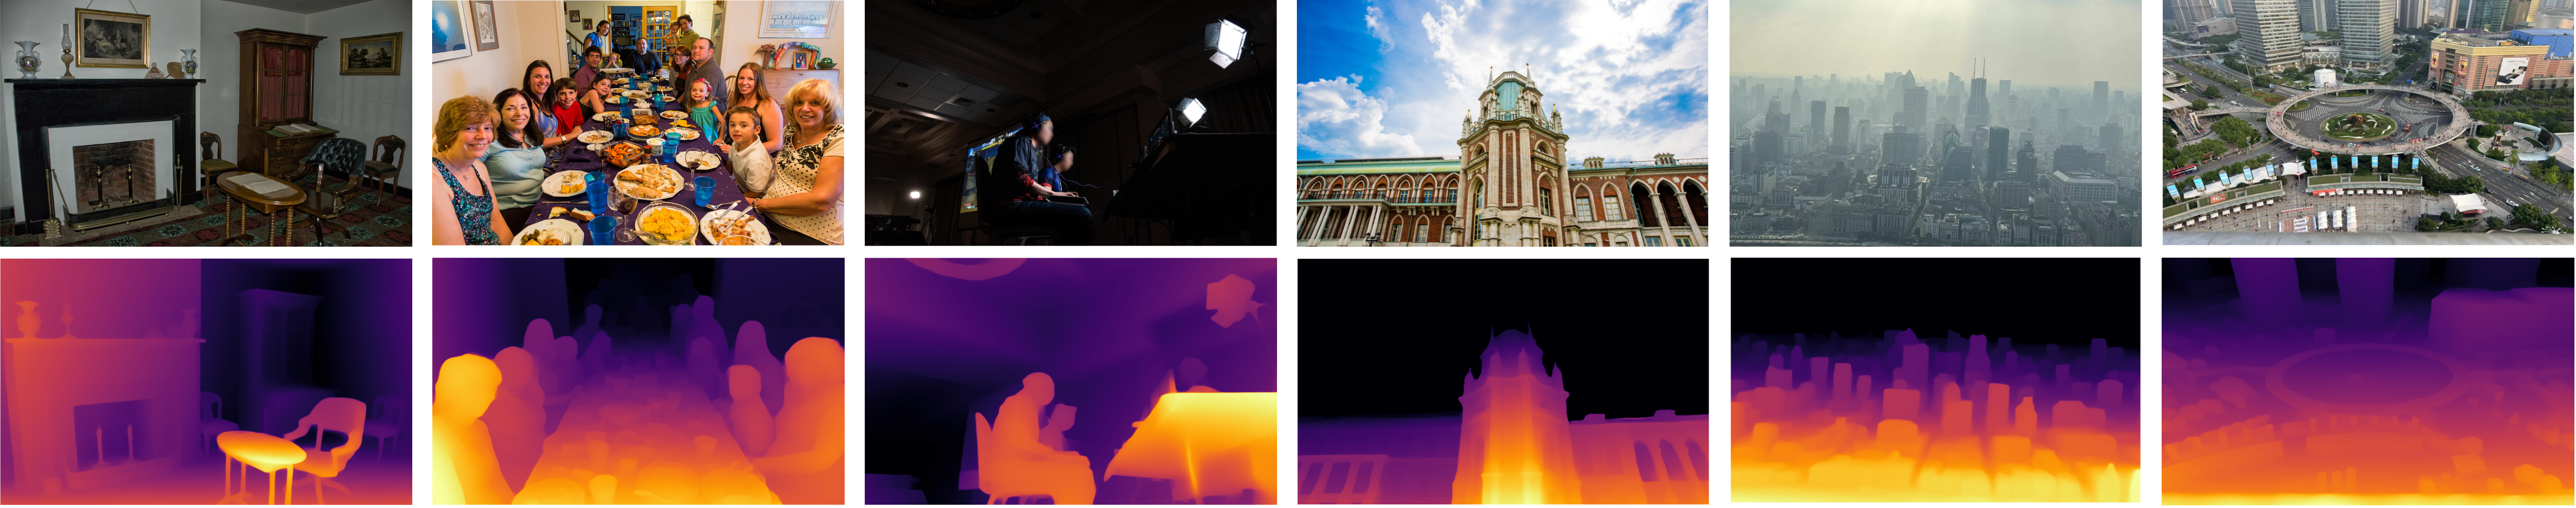
\includegraphics[width=1\textwidth]{17.jpg}
    \caption{Przykładowe wyniki działania modelu Depth Anything. Źródło: \cite{yang2024}}
    \label{depth-anything}
\end{figure}
W architekturze tego rozwiązania zastosowano koder wyodrębniający cechy obrazu wejściowego przygotowany na podstawie DINOv2 \cite{oquab2024} oraz dekoder DPT do regresji głębi. W pierwszej kolejności model "nauczyciela" uczony jest na zestawie danych oznaczonych. Następnie model ten wykorzystywany jest w celu oznaczenia zbioru danych nieoznaczonych, który razem z zestawem danych oznaczonych weźmie udział w procesie uczenia modelu "ucznia".
\begin{figure}[H]
    \centering
    
\includegraphics[width=1\textwidth]{18.jpg}
    \caption{Schemat architektury algorytmu Depth Anything. Źródło: \cite{yang2024}}
    \label{fig:depth-anything-schema}
\end{figure}
\begin{figure}[H]
    \centering
    \includegraphics[width=0.6\textwidth]{19.jpg}
    \caption{Zbiór zestawów danych uczących Depth Anything. Źródło: \cite{yang2024}}
    \label{fig:depth-anything-data}
\end{figure}
Osiągane wyniki w porównaniach przeprowadzonych na zbiorach danych testowych w sposób zdecydowany udowadniają tezę autorów dotyczącą zasadności skalowania zestawów uczących przy pomocy danych nieoznaczonych.
\begin{figure}[H]
    \centering
    \includegraphics[width=1\textwidth]{20.jpg}
    \caption{Porównanie rezultatów Depth Anything dokonane na podstawie zbioru NYUv2 (po lewej) i KITTI (po prawej). Źródło: \cite{yang2024}}
    \label{fig:depth-anything-results}
\end{figure}

\subsection{Metric3D}
Metoda Metric3D \cite{hu2024} adresuje dwa kluczowe problemy: estymację metrycznej głębokości i normalnych powierzchni z pojedynczego obrazu. Jest ona zaprojektowana z uwzględnieniem wysokiej generalizacji, w związku z czym bez dodatkowego dostrajania można ją wykorzystać w celu predykcji na obrazach prezentujących zróżnicowane sceny.
Głębokość metryczna pozwala na precyzyjne odwzorowanie rzeczywistego świata, podczas gdy normalne powierzchni zapewniają szczegółową geometrię lokalną.

Do trenowania modelu użyto dużego zestawu danych obejmującego 18 różnych zbiorów, które łącznie zawierają ponad 16 milionów obrazów. Zbiory te pochodzą z różnych typów scen, zarówno wewnętrznych jak i zewnętrznych, oraz obejmują różne modele kamer. Do testowania natomiast użyto zestawów danych 7 zestawów częściowo pokrywających się z zestawami uczącymi.

\begin{figure}[H]
    \centering
    \includegraphics[width=1\textwidth]{25.jpg}
    \caption{Uproszczony schemat architektury rozwiązania Metric3D. Źródło: \cite{hu2024}}
    \label{fig:metric3d-schema}
\end{figure}

Autorzy tej metody zastosowali w niej zarówno architekturę opartą o konwolucyjną sieć neuronową (UNet) jak i transformator (ViT i DPT jako dekoder), w zależności od konfiguracji metoda może korzystać z jednej z nich. Wyniki Metric3D na dzień opracowania bieżącego rozdziału ustanawiają nowy stan sztuki osiąganymi wynikami, które prezentuje poniższa tabela.
\begin{figure}[H]
    \centering
    \includegraphics[width=1\textwidth]{26.jpg}
    \caption{Porównanie rezultatów Metric3D do innych wiodących metod. Źródło: \cite{hu2024}}
    \label{fig:metric3d-results}
\end{figure}

\subsection{DistDepth}
Autorzy pracy prezentującej metodę DistDepth \cite{wu2022practical} zwracają uwagę na to, że dostępne obecnie metody skupiające się na obrazach przedstawiających ruch uliczny nie znajdują dobrego zastosowania w predykcji głebi na obrazach przedstawiających skomplikowane sceny wewnętrzne, szczególnie takie które na planie posiadają wiele gęsto ulokowanych przedmiotów. Proponują oni rozwiązanie składające się z dwóch części - estymatora struktur ze względnymi wartościami głębokości opartego o transformator wizyjny, którego wynik wraz z obrazem wejściowym wysyłany jest na wejście estymatora głębi opartego o konwolucyjną sieć neuronową trenowanego w sposób nienadzorowany. W ten sposób uzyskany model w czasie rzeczywistym wnioskuje głębię pojedynczego obrazu z wysoką generalizacją pośród scen wewnętrznych.
\begin{figure}[H]
    \centering
    \includegraphics[width=1\textwidth]{27.jpg}
    \caption{Schemat przedstawiający działanie algorytmu DistDepth. Źródło: \cite{wu2022practical}}
    \label{fig:distdepth-teaser}
\end{figure}
W celu nauczenia algorytmu DistDepth wykorzystano dwa autorskie zestawy danych - SimSIN zawierający 500 tysięcy symulowanych komputerowo obrazów scen wewnętrznych w postaci par stereo (ponieważ uczenie odbywa się w sposób nienadzorowany, sceny nie zawierają żadnej informacji o głębi) oraz UniSIN zawierający 200 tysięcy obrazów scen predstawiających wnętrza uniwersytetu zarejestrowanych za pomocą urządzenia ZED 2I \cite{ZED2I}.
\begin{figure}[H]
    \centering
    \includegraphics[width=0.8\textwidth]{28.jpg}
    \caption{Porównanie wyników z innymi rozwiązaniami wykonane na zestawie NYU v2. Źródło: \cite{wu2022practical}}
    \label{fig:distdepth-results}
\end{figure}

\subsection{GCNDepth}
Wykorzystujący architekturę grafowej konwolucyjnej sieci neuronowej \cite{GNNBook2022} model GCNDepth \cite{masoumian2021gcndepth} oferuje według twórców 89\% skuteczność na publicznie dostępnych zbiorach KITTI i Make3D, redukując jednocześnie o 40\% ilość trenowanych parametrów sieci w porównaniu z innymi obecnymi algorytmami. Model ten koncentruje się na scenach plenerowych, szczegónie na ruchu ulicznym ze względu na charakterystykę obrazów trenujących. Precyzując architektura składa się z dwóch głównych komponentów: sieci DepthNet odpowiedzialnej za przewidywanie map głębokości oraz sieci PoseNet odpowiedzialnej za przewidywanie pozy aparatu między kolejnymi klatkami wideo ze względu na nienadzorowane uczenie algorytmu. Poniższa ilustracja zawiera schemat opisanej architektury.
\begin{figure}[H]
    \centering
    \includegraphics[width=0.8\textwidth]{29.jpg}
    \caption{Schemat przedstawiający architekturę modelu GCNDepth. Źródło: \cite{GNNBook2022}}
    \label{fig:gcn-schema}
\end{figure}
Zbiór trenujący modelu GCNDepth stanowi 200 nagrań wideo ruchu ulicznego w świetle dziennym z publicznego zestawu KITTI. Na tym zestawie oraz na Make3D autorzy dokonali testów uzyskanego modelu. Wyniki w porównaniu do podobnych rozwiązań przedstawione zostały w postaci tabeli.
\begin{figure}[H]
    \centering
    \includegraphics[width=0.8\textwidth]{30.jpg}
    \caption{Wyniki GCNDepth uzyskane na zestawie KITTI w porównaniu z podobnymi rozwiązaniami. Źródło: \cite{GNNBook2022}}
    \label{fig:gcn-results}
\end{figure}


\subsection{M4Depth}
Metoda M4Depth \cite{fonder2023technique} została zaprojektowana z myślą o bezzałogowych statkach powietrznych. Jej autorzy podkreślają jak istotne jest oszacowanie niepewności obok estymacji głębokości w tym konkretnym zastosowaniu. Ponadto w tak niewielkich statkach powietrznych waga stanowi kwestię kluczową, przez co jeden obiektyw zamiast dwóch jest zdecydowanie lepszym wyborem. Metoda ta ma być według autorów ponad 2 razy szybsza przy zachowaniu podobnej dokładności, co również nie pozostaje obojętne w kontekście lotów dronem.
\begin{figure}[H]
    \centering
    \includegraphics[width=0.7\textwidth]{31.jpg}
    \caption{Przykłady działania modelu M4Depth wraz z estymacją niepewności. Źródło: \cite{fonder2023technique}}
    \label{fig:m4d-example}
\end{figure}
W zależności od zastosowanej funkcji straty - jednej z dwóch - wykorzystanej w procesie uczenia model przyjmuje nazwę M4Depth+U\textsubscript{$\rho$} lub M4Depth+U\textsubscript{z}.
Model został wytrenowany na zbiorze Mid-Air \cite{fonder2019midair}, czyli syntetycznych obrazach stanowiących wizualizacje lotu dronem zawierających między innymi informację o głębi sceny. Testy dokonano natomiast przy użyciu zbiorów Mid-Air, KITTI oraz TartanAir \cite{wang2020tartanair}. Poniższa tabela zawiera porównanie z innymi modelami, należy zwrócić uwagę na czas wymagany na estymację przez poszczególne algorytmy.
\begin{figure}[H]
    \centering
    \includegraphics[width=0.7\textwidth]{32.jpg}
    \caption{Porównanie wyników działania metody M4Depth na zbiorze KITTI. Źródło: \cite{fonder2023technique}}
    \label{fig:m4d-comparison}
\end{figure}

\subsection{IndoorDepth}
IndoorDepth \cite{fan2023deeper} to model głębokiej sieci neuronowej zaprojektowany do estymacji głębokości w scenach wewnętrznych. Podobnie jak GCNDepth, IndoorDepth wykorzystuje uczenie samonadzorowane, co eliminuje potrzebę etykietowanych danych głębokościowych, wykorzystując sekwencje obrazów jako sygnał nadzoru. Architektura modelu to konwolucyjna sieć neuronowa z enkoderem i dekoderem, używanymi do estymacji pozycji kamery i głębokości oraz ulepszonej funkcji SSIM (od ang. structural similarity), która lepiej radzi sobie z regionami o niskiej teksturze.
\begin{figure}[H]
    \centering
    \includegraphics[width=1\textwidth]{33.jpg}
    \caption{Schemat architektury modelu IndoorDepth. Źródło: \cite{fan2023deeper}}
    \label{fig:indoordepth-architecture}
\end{figure}
Do trenowania modelu użyto zestawu danych NYUv2, składającego się z 47 tysięcy obrazów, wybranych na podstawie próbkowania co 5 klatek z surowego zestawu danych. Do testowania modelu wykorzystano oficjalny zestaw 654 obrazów z danymi o głębi z NYUv2 oraz dodatkowy zestaw ScanNet, użyty do oceny zdolności generalizacji modelu na nowych scenach wewnętrznych.
\begin{figure}[H]
    \centering
    \includegraphics[width=0.75\textwidth]{34.jpg}
    \caption{Porównanie wyników działania metody IndoorDepth na zbiorze NYUv2. Źródło: \cite{fan2023deeper}}
    \label{fig:indoordepth-results}
\end{figure}

\subsection{SQLdepth}
Model SQLdepth \cite{wang2023sqldepth} jest głęboką siecią neuronową zaprojektowaną do estymacji głębokości obrazu w sposób samonadzorowany. Model SQLdepth operuje na scenach zewnętrznych, wykorzystując zestaw danych KITTI zawierający sekwencje stereo obrazów. Architektura modelu opiera się na konwolucyjnej sieci neuronowej z enkoderem-dekoderem, wspieranej warstwą Self Query Layer (SQL), która poprawia dokładność przewidywania głębokości.
\begin{figure}[H]
    \centering
    \includegraphics[width=1\textwidth]{35.jpg}
    \caption{Schemat architektury modelu SQLdepth. Źródło: \cite{wang2023sqldepth}}
    \label{fig:sqldepth-architecture}
\end{figure}
Podczas treningu model wykorzystuje pary stereo jako główne źródło nadzoru. Do uczenia modelu użyto około 26 tysięcy obrazów z zestawu KITTI, natomiast do testowania wykorzystano 697 obrazów z tego samego zestawu. Model był również ewaluowany na zestawach danych Cityscapes, obejmujących liczne ruchome obiekty oraz Make3D, który został użyty do oceny zdolności generalizacji modelu na wcześniej niewidzianych obrazach.
\begin{figure}[H]
    \centering
    \includegraphics[width=0.95\textwidth]{36.jpg}
    \caption{Porównanie wyników działania metody IndoorDepth na zbiorze KITTI. Źródło: \cite{wang2023sqldepth}}
    \label{fig:sqldepth-results}
\end{figure}


\subsection{Podsumowanie}
Przedstawione algorytmy można skategoryzować ze względu na rodzaj architektury, charakterystykę zestawów uczących i charakterystykę wyników. Poniższa tabela zawiera krótkie podsumowanie.
\begin{table}[H]
    \centering
    \caption{Podsumowanie przedstawionych modeli percepcji głębi.}
    \vspace{0.1cm}
    \resizebox{\textwidth}{!}{%
        \begin{tabular}{ |l|p{2cm}|p{2cm}|p{5cm}|p{5cm}|r| }
        \hline
        Nazwa & Architektura & Sposób uczenia & Zestawy uczące & Zestawy do oceny \\
        \hline \hline
        AdelaiDepth &
        konwolucyjna sieć neuronowa &
        nadzorowane &
        \begin{itemize} 
            \item Taskonomy,
            \item 3D Ken Burns, 
            \item DIML, 
            \item Holopix50K, 
            \item HRWSI. 
        \end{itemize} &
        \begin{itemize} 
            \item NYU depth V2,
            \item KITTI,
            \item ScanNet,
            \item DIODE,
            \item ETH3D,
            \item Sintel,
            \item OASIS,
            \item YouTube3D,
            \item RedWeb,
            \item iBims-1. 
        \end{itemize}\\
        \hline
        MetaPrompt-SD &
        konwolucyjna sieć neuronowa &
        nadzorowane &
        \begin{itemize} 
            \item NYU depth V2,
            \item KITTI.
        \end{itemize} & 
        Zestawy tożsame z uczącymi.\\
        \hline
        EVP &
        konwolucyjna sieć neuronowa &
        nadzorowane &
        \begin{itemize} 
            \item NYU depth V2,
            \item KITTI.
        \end{itemize} & 
        Zestawy tożsame z uczącymi.\\
        \hline
        ZoeDepth &
        konwolucyjna sieć neuronowa &
        nadzorowane i częściowo nadzorowane &
        \begin{itemize} 
            \item NYU depth V2,
            \item KITTI,
            \item HRWSI,
            \item BlendedMVS,
            \item ReDWeb,
            \item DIML-Indoor,
            \item 3D Movies,
            \item MegaDepth,
            \item WSVD,
            \item TartanAir,
            \item ApolloScape,
            \item IRS.
        \end{itemize} & 
        \begin{itemize} 
            \item SUN RGB-D,
            \item iBims,
            \item DIODE,
            \item HyperSim,
            \item DDAD,
            \item DIML,
            \item Virtual KITTI 2.
        \end{itemize}\\
        \hline
        UniDepth &
        W zależności od konfiguracji konwolucyjna sieć neuronowa lub transformator. &
        nadzorowane &
        \begin{itemize}
        \item Argoverse2,
        \item Waymo,
        \item DrivingStereo,
        \item Cityscapes,
        \item BDD100K,
        \item MapillaryPSD,
        \item A2D2,
        \item ScanNet,
        \item Taskonomy.
        \end{itemize} & 
        \begin{itemize} 
            \item SUN-RGBD,
            \item Diode Indoor,
            \item IBims-1,
            \item VOID,
            \item HAMMER,
            \item ETH-3D,
            \item nuScenes,
            \item DDAD,
            \item NYU-Depth V2,
            \item KITTI.
        \end{itemize}\\
        \hline
        \end{tabular}%
    }
    \label{tabela_podsumowanie_algorytmy}
\end{table}

\begin{table}[H]
    \centering
    \vspace{0.1cm}
    \resizebox{\textwidth}{!}{%
        \begin{tabular}{ |l|p{2cm}|p{3cm}|p{5cm}|p{5cm}|r| }
        \hline
        Depth Anything &
        transormator &
        częściowo nadzorowane &
        \begin{itemize}
        \item zbiory oznaczone
            \begin{itemize}
                \item BlendedMVS,
                \item DIML,
                \item HRWSI,
                \item IRS,
                \item MegaDepth,
                \item TartanAir.
            \end{itemize}
        \item zbiory nieoznaczone
            \begin{itemize}
                \item BDD100K,
                \item Google Landmarks,
                \item ImageNet-21K,
                \item LSUN,
                \item Objects365,
                \item Open Images V7,
                \item Places365,
                \item OSA-1B.
            \end{itemize}
        \end{itemize} & 
        \begin{itemize} 
            \item zbiory do oceny predykcji głębi relatywnej
            \begin{itemize} 
                \item NYU depth V2,
                \item KITTI,
                \item Sintel,
                \item DDAD,
                \item ETH3D,
                \item DIODE,
            \end{itemize}
            \item zbiory do oceny predykcji głębi metrycznej
            \begin{itemize} 
                \item SUN RGB-D,
                \item iBims-1,
                \item HyperSim,
                \item Virtual KITTI 2,
                \item DIODE Outdoor.
            \end{itemize}
        \end{itemize}\\
        \hline
        Metric3D &
        W zależności od konfiguracji konwolucyjna sieć neuronowa lub transformator. &
        nadzorowane &
        \begin{itemize}
            \item DDAD,
            \item Lyft,
            \item Driving Stereo (DS),
            \item DIML,
            \item Arogoverse2,
            \item Cityscapes,
            \item DSEC,
            \item Mapillary PSD,
            \item Pandaset,
            \item UASOL,
            \item Virtual KITTI,
            \item Waymo,
            \item Matterport3d,
            \item Taskonomy,
            \item Replica,
            \item ScanNet,
            \item HM3d,
            \item Hypersim.
        \end{itemize} & 
        \begin{itemize}
            \item NYU,
            \item KITTI,
            \item ScanNet,
            \item NuScenes (NS),
            \item ETH3D,
            \item DIODE,
            \item iBims-1.
        \end{itemize}\\
        \hline
        DistDepth &
        Konwolucyjna sieć neuronowa i transformator. &
        nienadzorowane &
        \begin{itemize}
            \item SimSIN,
            \item UniSIN.
        \end{itemize} & 
        \begin{itemize}
            \item VA,
            \item NYUv2,
            \item Hypersim.
        \end{itemize}\\
        \hline
        GCNDepth &
        Grafowa i nawracająca sieć neuronowa &
        nienadzorowane &
        \begin{itemize}
            \item KITTI
        \end{itemize} & 
        \begin{itemize}
            \item KITTI,
            \item Make3D.
        \end{itemize}\\
        \hline
        M4Depth &
        Konwolucyjna sieć neuronowa &
        nadzorowane &
        \begin{itemize}
            \item Mid-Air
        \end{itemize} & 
        \begin{itemize}
            \item Mid-Air,
            \item KITTI,
            \item TartanAir.
        \end{itemize}\\
        \hline
        IndoorDepth &
        Konwolucyjna sieć neuronowa &
        nienadzorowane &
        \begin{itemize}
            \item NYUv2
        \end{itemize} & 
        \begin{itemize}
            \item NYUv2,
            \item ScanNet.
        \end{itemize}\\
        \hline
        SQLdepth &
        Konwolucyjna sieć neuronowa &
        nienadzorowane &
        \begin{itemize}
            \item KITTI
        \end{itemize} & 
        \begin{itemize}
            \item KITTI,
            \item Cityscapes,
            \item Make3D.
        \end{itemize}\\
        \hline
        \end{tabular}%
    }
    \label{tabela_podsumowanie_algorytmy_2}
\end{table}

\section{Zbiory danych}
\subsection{KITTI (Karlsruhe Institute of Technology and Toyota Technological Institute)}
Wiodącym zestawem danych używanym do trenowania i oceny algorytmów percepcji głębi jest opracowany przez niemiecki Instytut Technologii Karlsruhe'a oraz amerykański Instytut Technologii Toyota zbiór KITTI\footnote{Nazwa KITTI jest skrótem nazw instytutów przez które zbiór został opracowany.} \cite{geiger2012}. Zawiera on 93 tysiące obrazów RGB-D zarejestrowanych przy pomocy autorskiej platformy jezdnej Annieway składającej się z lasera firmy Velodyne \cite{Velodyne}, kamer kolorowych i monochromatycznych oraz systemu GPS zamontowanych na samochodzie osobowym. Obrazy należące do tego zbioru podzielone zostały na pięć kategorii: drogi, miasta, osiedla, kampus i osoby. Prezentują one zatem sceny zewnętrzne.
\begin{figure}[H]
    \centering
    \includegraphics[width=0.4\textwidth]{23.jpg}
    \caption{Rejestrująca platforma jezdna użyta w przygotowaniu zbioru KITTI. Źródło: \cite{geiger2012}}
    \label{fig:kitti-annieway}
\end{figure}
\subsection{NYUv2 (NYU-Depth V2)}
Drugim najczęściej wykorzystywanym zestawem obrazów jest NYUv2 przedstawiony w 2012 r. w \cite{couprie2013}. Zestaw ten składa się z 407024 obrazów RGB z odpowiadającymi im mapami głębi przygotowanymi przy użyciu urządzenia Microsoft Kinect. Autorzy skategoryzowali obrazy w zbiorze na następujące kategorie: piwnice, łazienki, sypialnie, księgarnia, kawiarnia, salony, jadalnie, sklepy meblowe, biura, kuchnie, biblioteki, bawialnie i inne. Obrazy przygotowane przez autorów NYUv2 przedstawiają wyłącznie sceny wewnątrz budynków. Niniejszy zestaw jest również wykorzystywany w dziedzinie segmentacji obrazu ze względu na przygotowane oznaczenie obrazów.
\subsection{DIODE (Dense Indoor and Outdoor Depth)}
Zbiór DIODE \cite{vasiljevic2019} jest wyjątkowy na tle konkurencji przez wzgląd na różnorodność scen. Jest bowiem pierwszym publicznie dostępnym zestawem obrazów prezentujących sceny zewnętrzne i wewnętrzne. Większa różnorodność scen pozwala na uzyskanie lepszych wyników na płaszczyźnie generalizacji modeli percepcji głębi. Na ten zbiór składa się 8574 obrazów scen wewnętrznych oraz 16884 obrazów scen zewnętrznych zarejestrowanych za pomocą tego samego urządzenia - skanera FARO Focus S350. Przygotowane przez twórców zbioru porównanie z podobnymi zestawami wskazuje na wysoką dokładność i zasięg zastosowanej aparatury.
\begin{figure}[H]
    \centering
    \includegraphics[width=0.8\textwidth]{24.jpg}
    \caption{Porównanie statystyk zbioru DIODE z innymi popularnymi zbiorami danych. Źródło: \cite{vasiljevic2019}}
    \label{fig:diode-comparison}
\end{figure}
\subsection{SUN RGB-D}
Głównym założeniem zestawu SUN RGB-D \cite{song2015} jest dostarczenie danych dla modeli interpretujących trójwymiarowe sceny. Składa się on z 10335 obrazów pomieszczeń wewnętrznych z mapami głębi pochodzącymi z sensorów Intel Realsense, Asus Xtion i obu wersji Microsoft Kinect. Na rzeczone obrazy zostały naniesione trójwymiarowe oznaczenia widniejących przedmiotów. Z powodu odmiennego przeznaczenia, zbiór ten jest często wykorzystywany w celu oceny działania modeli percepcji głębi.
\subsection{Matterport3D}
W 2017 r. firma Matterport zaprezentowała zestaw danych Matterport3D \cite{chang2017} przygotowany przy pomocy autorskiego urządzenia rejestrującego. Zestaw składa się z 10800 zdjęć panoramicznych złożonych z 194400 obrazów z odpowiadającą im mapą głębi. Zdjęcia w zbiorze przedstawiają 90 scen przedstawiających wnętrza budynków. 
\subsection{DDAD (Dense Depth for Autonomous Driving)}
Zestaw DDAD \cite{guizilini2020} został stworzony przez Toyota Research Institute. Zawiera 17050 obrazów treningowych i 4150 obrazów do oceny modelu, w tym zróżnicowane próbki scen miejskich i autostradowych z całego świata nagrane przez flotę samochodów autonomicznych wyposażonych w kamery i lasery LIDAR Luminar-H2. Wykorzystywany jest głównie do ewaluacji i rozwijania metod estymacji głębi w prowadzeniu pojazdów. Zestaw DDAD został wykorzystany do przetrenowania modelu PackNet tego samego autorstwa, nie osiąga on jednak wyników porównywalnych do wybranych w niniejszej pracy modeli.

\subsection{Podsumowanie}
Wykazane w niniejszym rozdziale zestawy danych przyczyniły się w znacznej mierze do rozwoju metod predykcji głębi. Rozbieżność ich cech z kolei przyczynia się pozytywnie do generalizacji modeli. Poniższa tabela stanowi wykaz przedstawionych zestawów z podziałem na charakterystykę scen, liczebność i urządzenie rejestrujące.
\begin{table}[H]
    \centering
    \caption{Podsumowanie przedstawionych zbiorów danych używanych przez algorytmy percepcji głębi.}
    \vspace{0.1cm}
    \resizebox{\textwidth}{!}{%
        \begin{tabular}{ |p{3cm}|p{3cm}|p{5cm}|p{5cm}|r| }
        \hline
        Nazwa & Charakterystyka obrazów & Liczebność zbioru & Urządzenie rejestrujące \\
        \hline \hline
        KITTI &
        sceny zewnętrzne & 
        93000 &
        Skaner laserowy Velodyne \cite{Velodyne} i system lokalizacji GPS. \\
        \hline
        NYUv2 &
        sceny wewnętrzne & 
        407024 &
        Microsoft Kinect \\
        \hline
        DIODE &
        sceny zewnętrzne i wewnętrzne & 
        25458 &
        Skaner FARO Focus S350 \\
        \hline
        SUN RGB-D &
        sceny wewnętrzne & 
        10335 &
        Intel RealSense 3D, Asus Xtion LIVE PRO i Microsoft
Kinect. \\
        \hline
        Matterport3D &
        sceny wewnętrzne & 
        194400 &
        Autorska konstrukcja Matterport.  \\
        \hline
        DDAD &
        sceny zewnętrzne & 
        21200 &
        Luminar-H2  \\
        \hline
        \end{tabular}%
    }
    \label{tabela_podsumowanie_zbiory}
\end{table}
    \chapter{Przedstawienie zastosowanych narzędzi}\label{chap:przedstawienie_zastosowanych_narzędzi}

\section{Język programowania}
Obecnie, Python, język programowania wysokiego poziomu ogólnego przeznaczenia, wprowadzony w 1991 roku przez Guido van Rossum’a \cite{Python}, dominuje w dziedzinie sztucznej inteligencji. Charakteryzuje się on prostą składnią, która ułatwia naukę i stosowanie w praktyce, co czyni go szczególnie popularnym wśród inżynierów danych. Python jest ceniony za wsparcie licznych bibliotek specjalizujących się w przetwarzaniu danych i uczeniu maszynowym, jak również za otwartoźródłowy charakter, co umożliwia szeroką współpracę w społeczności naukowej. W pracy przedstawione zostały modele wykorzystujące język Python w połączeniu z biblioteką PyTorch \cite{paszke2019}, która jest rozwijana na bazie Torch i umożliwia efektywne budowanie oraz trenowanie modeli głębokiego uczenia z użyciem procesora graficznego.

\section{Platforma obliczeniowa}
W celu uruchomienia analizowanych metod neuronowych wizyjnych algorytmów percepcji głębi, wykorzystano platformę obliczeniową Google Colab. Jest to platforma sieciowa, która umożliwia uruchamianie skryptów w języku Python bezpośrednio w przeglądarce, co jest szczególnie korzystne w kontekście prac badawczych i edukacyjnych\footnote{\href{https://colab.google/}{https://colab.google/}}. Platforma ta opiera się na technologii Jupyter Notebook, co umożliwia interaktywne programowanie i wizualizację danych\footnote{\href{https://jupyter.org/}{https://jupyter.org/}}.

Google Colab oferuje dostęp do mocnych zasobów obliczeniowych, w tym do procesorów graficznych (GPU) i jednostek przetwarzania tensorów (TPU), które są kluczowe przy trenowaniu skomplikowanych modeli głębokiego uczenia. Użytkownicy mogą łatwo skalować użycie zasobów w zależności od potrzeb danego algorytmu, co znacząco redukuje czas i koszt przetwarzania. Dostępność tych zasobów przez platformę internetową umożliwia również łatwe udostępnianie wyników i współpracę w ramach zespołów rozproszonych geograficznie.

W kontekście przeprowadzonej analizy, Google Colab okazał się być nieocenionym narzędziem, które pozwoliło na efektywne wykonanie i analizę algorytmów percepcji głębi. Możliwość wyświetlania wyników bezpośrednio w przeglądarce internetowej znacząco ułatwiła proces badawczy i pozwoliła na dynamiczne dopasowanie parametrów modelu w odpowiedzi na obserwowane wyniki.

\section{Zestawy danych}
Niewątpliwie kluczową rolę w procesie analizy porównawczej algorytmów percepcji głębi odgrywają odpowiednio dobrane zestawy danych. Wiele metod jest testowanych przez ich twórców na zbiorach tożsamych do tych na których były uczone. Powoduje to brak poprawnej oceny zdolności do generalizacji danego algorytmu na niewidzianych podczas uczenia scenach. W celu uniknięcia tego typu błędów, w niniejszej pracy do analizy algorytmów wykorzystano zestawy danych, które są dostępne publicznie, jednak nie zostały wykorzystane w procesie uczenia żadnego analizowanego modelu.

Ponadto każda z metod została zweryfikowana na autorskim zestawie danych. Został on przygotowany na potrzeby niniejszej pracy za pomocą technologii LIDAR stanowiącej wyposażenie urządzenia iPhone 15 Pro \cite{chase2022apple}. Zastosowany w rzeczonym urządzeniu skaner emituje matrycę zawierającą 8x8 punktów która jest podzielona na siatki 3x3 co daje łącznie 576 punktów. Maksymalny zasięg tego skanera to 5 metrów. Fotografie i skany zostały wykonane w otwartych przestrzeniach - głównie we Wrocławskim Ogrodzie Zoologicznym. Obrazy RGB wraz z odpowiadającymi im mapami głębi pochodzącymi z autorskiego zestawu są dostępne w załączniku do pracy.
\begin{figure}[H]
    \centering
    \includegraphics[width=0.55\textwidth]{45.jpg}
    \caption{a) emitowana matryca punktów b) umiejscowienie skanera w urządzeniu c) przykładowy model 3D wykonany przy użycciu skanera d) przykład implementacji w oprogramowaniu. Źródło: \cite{luetzenburg2021evaluation}}
    \label{fig:iphone-lidar}
\end{figure}

\section{Narzędzia do analizy i wizualizacji}
Algorytmy percepcji głębi, które bazują na sieciach neuronowych, są złożonymi modelami, wymagającymi odpowiednich technik analitycznych do ich oceny i porównania. W związku z tym, odpowiedni dobór narzędzi ma kluczowe znaczenie dla poprawności i efektywności przeprowadzanych analiz.

W ramach języka programowania Python wykorzystany został bogaty ekosystem bibliotek, takich jak NumPy, pandas i OpenCV, umożliwiają one efektywną manipulację danymi, wykonywanie skomplikowanych obliczeń oraz analiz statystycznych szczególnie w kontekście widzenia komputerowego. Matplotlib to natomiast podstawowa biblioteka do tworzenia graficznych wizualizacji danych. Dzięki niej możliwe było tworzenie wykresów prezentujących wyniki analizy oraz porównania wydajności różnych algorytmów.

W celu trenowania sieci oraz uruchomienia predykcji na zbiorach przygotowanych do analizy zastosowana została platforma PyTorch - najpopularniejsza platforma do tworzenia i trenowania modeli głębokiego uczenia. Oferuje ona wsparcie dla zaawansowanych architektur sieci neuronowych oraz narzędzi do ich optymalizacji i oceny.

Wszystkie wymienione narzędzia uruchomione zostały na platformie Google Colab w środowisku Jupyter Notebook. Dobór odpowiednich narzędzi do analizy i wizualizacji danych jest kluczowy dla skutecznego przeprowadzenia porównania neuronowych algorytmów percepcji głębi. Wykorzystane narzędzia zapewniły solidne podstawy dla przeprowadzenia kompleksowej analizy. Dzięki nim możliwe było zarówno efektywne przetwarzanie danych, jak i klarowne prezentowanie wyników, co znacząco wpłynęło na jakość i przejrzystość przeprowadzonych badań.
\begin{figure}[H]
    \centering
    \includegraphics[width=1\textwidth]{46.jpg}
    \caption{Okno przeglądarki wyświetlające środowisko Google Colab.}
    \label{fig:google-colab}
\end{figure}

    \chapter{Zbiór danych do analizy porównawczej}\label{chap:zbiór_danych_do_analizy_porównawczej}

    \chapter{Metodologia - opis kryteriów oceny algorytmów}\label{chap:metodologia}

    \chapter{Analiza i wyniki}\label{chap:analiza_i_wyniki}

    \chapter{Podsumowanie i wnioski}\label{chap:podsumowanie_i_wnioski}


    % Bibliografia - musi być
    % Bibliography - must exist
    \bibliografia

    % Strony końcowe - można zakomentować, jeśli zbędne
    % Additional pages - comment out if not needed
    
    % Wykaz symboli i skrótów - patrz opis w tekście przykładowym
    \acronymslist
    % Spis rysunków
    \listoffigures
    % Spis tabel
    \listoftables
    % Załączniki (plik appendices.tex)
    \załączniki
\end{document}
%%%%%%%%%%%%%%%%%%%%%%%%%%%%%%%%%%%%%%%%%%%%%%%%%%%%%%%%%%%%%%%%%%%%%%%%%%%

